%%% Local Variables: 
%%% coding: utf-8
%%% mode: latex
%%% TeX-engine: xetex
%%% End: 

\documentclass[hide notes,intlimits]{beamer}
\mode<presentation>
{
  \usetheme[footline]{PISMshade}
  \setbeamercovered{transparent}
}

% load packages
\usepackage{media9}
\usepackage[english]{babel}
\usepackage[multidot]{grffile}

\usepackage{tikz}
\usetikzlibrary{shapes,arrows}
\usetikzlibrary{shadows}

\definecolor{dark red}{HTML}{E41A1C}
\definecolor{dark green}{HTML}{4DAF4A}
\definecolor{dark violet}{HTML}{984EA3}
\definecolor{dark blue}{HTML}{084594}
\definecolor{dark orange}{HTML}{FF7F00}
\definecolor{light blue}{HTML}{377EB8}
\definecolor{light red}{HTML}{FB9A99}
\definecolor{light violet}{HTML}{CAB2D6}

\setbeamercolor{boxed}{fg=black,bg=light blue!25}
\graphicspath{{figures/}{../figures/}{../figures_2018_08/}{../2022_04_igs/figures/}{../2021_09_cph/figures/}{../2021_11_geo/figures/}}


\newcommand{\jl}{[\![}
\newcommand{\jr}{]\!\hskip 0.003cm ]}
\newcommand{\bpsi}{\boldsymbol{\psi}}
\newcommand{\bPsi}{\boldsymbol{\Psi}}
\newcommand{\bphi}{\boldsymbol{\phi}}
\newcommand{\bPhi}{\boldsymbol{\Phi}}
\newcommand{\bn}{\mathbf{n}}
\newcommand{\bq}{\mathbf{q}}
\newcommand{\bv}{\mathbf{v}}
\newcommand{\D}{\,\mathrm{d}}
\newcommand{\Tsnow}{T_{\text{snow}}}
\newcommand{\Hatm}{H_{\text l}^{\text{atm}}}

\newcommand{\mathtext}[1]{\mathsf{#1}}

% title page
\title[Ice sheet modeling] % (optional, use only with long paper titles)
{The break-up of Sermeq Kujalleq\\(Jakobshavn Isbr{\ae})}
\author[Aschwanden] % (optional, use only with lots of authors)
{\textbf{Andy Aschwanden}, Doug Brinkerhoff\\ and others}
\institute{Geophysical Institute, University of Alaska Fairbanks}

% - Give the names in the same order as the appear in the paper.
% - Use the \inst{?} command only if the authors have different
%   affiliation.

% - Use the \inst command only if there are several affiliations.
% - Keep it simple, no one is interested in your street address.
 \titlegraphic{\vskip-.5cm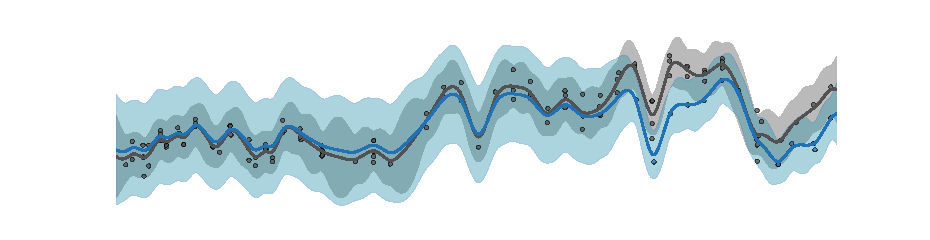
\includegraphics[height=3cm]{jib_temperature_forcing_1980_2020_green}}

 
\date{}


\subject{Incredible sea-level projections}

\begin{document}


\setbeamertemplate{background canvas}
  {
}


\setbeamertemplate{background canvas}
  {
     \tikz{\node[inner sep=0pt,opacity=1.0] {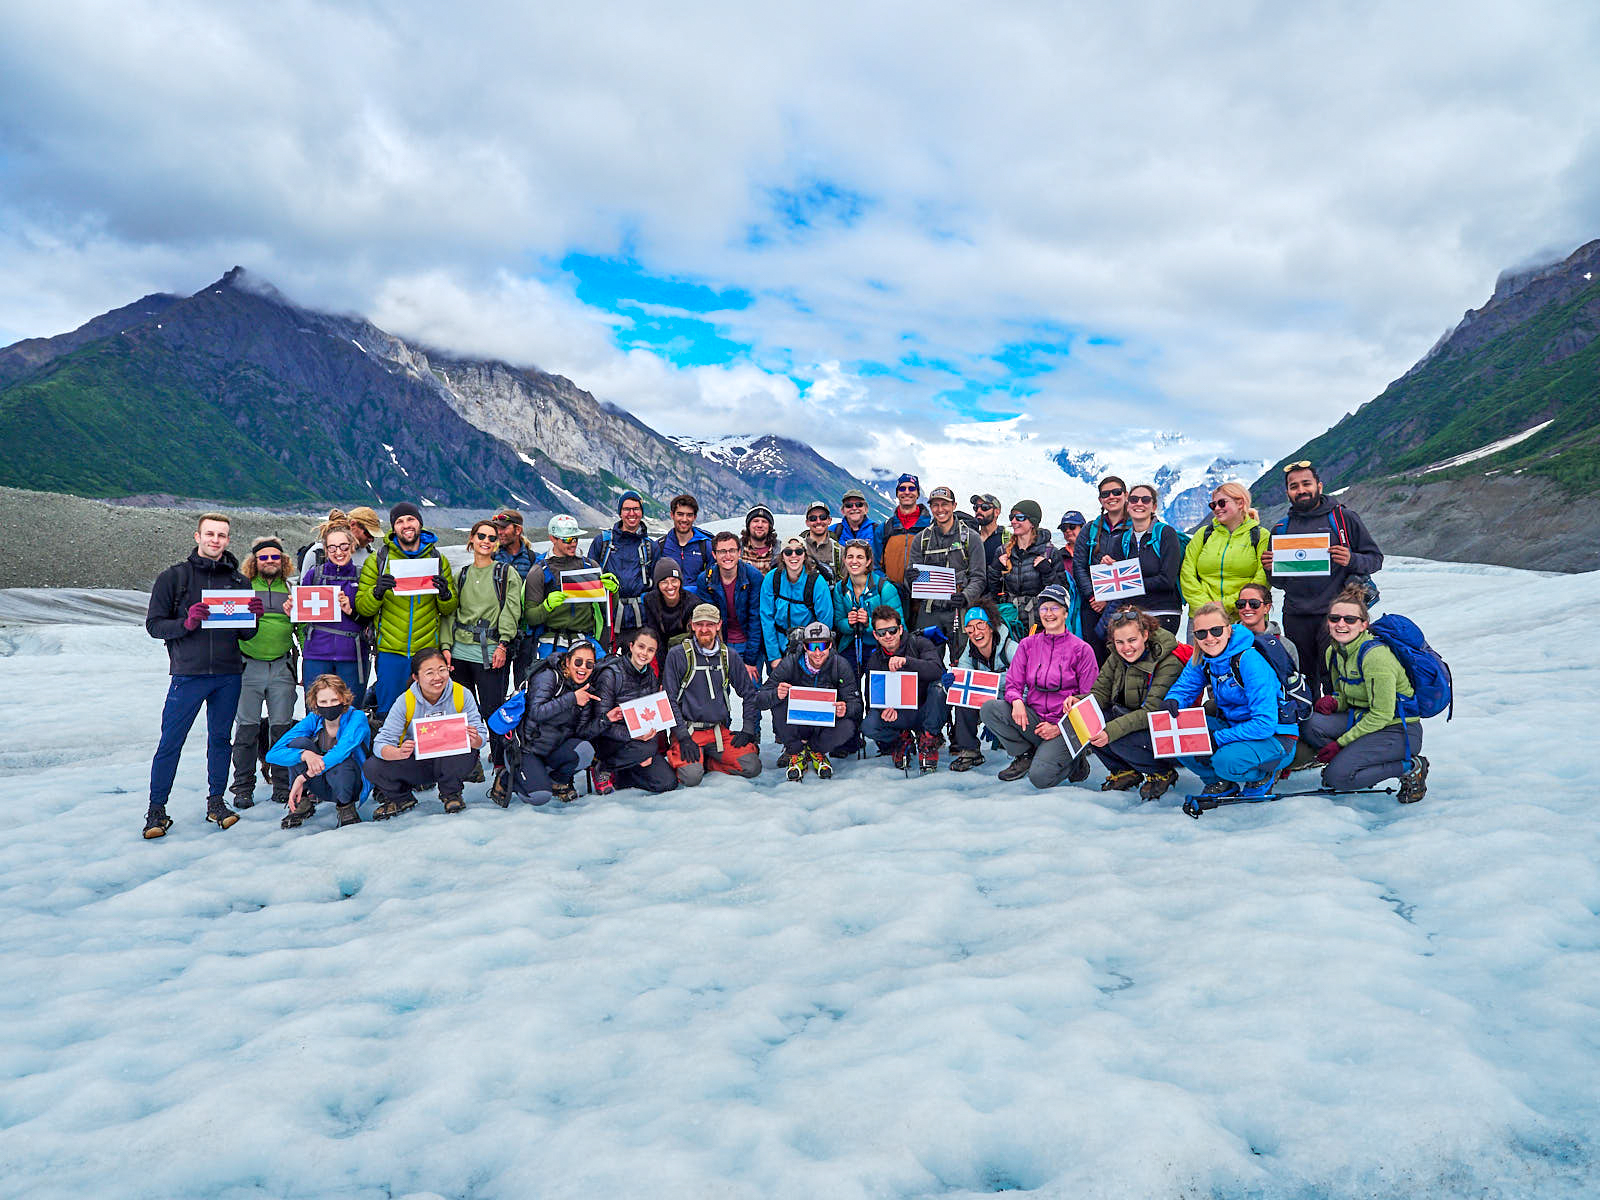
\includegraphics[width=\paperwidth]{mccarthy-summer-school-2022-group}};}
}

\begin{frame}[plain]
\end{frame}

\setbeamertemplate{background canvas}
  {
     \tikz{\node[inner sep=0pt,opacity=1.0] {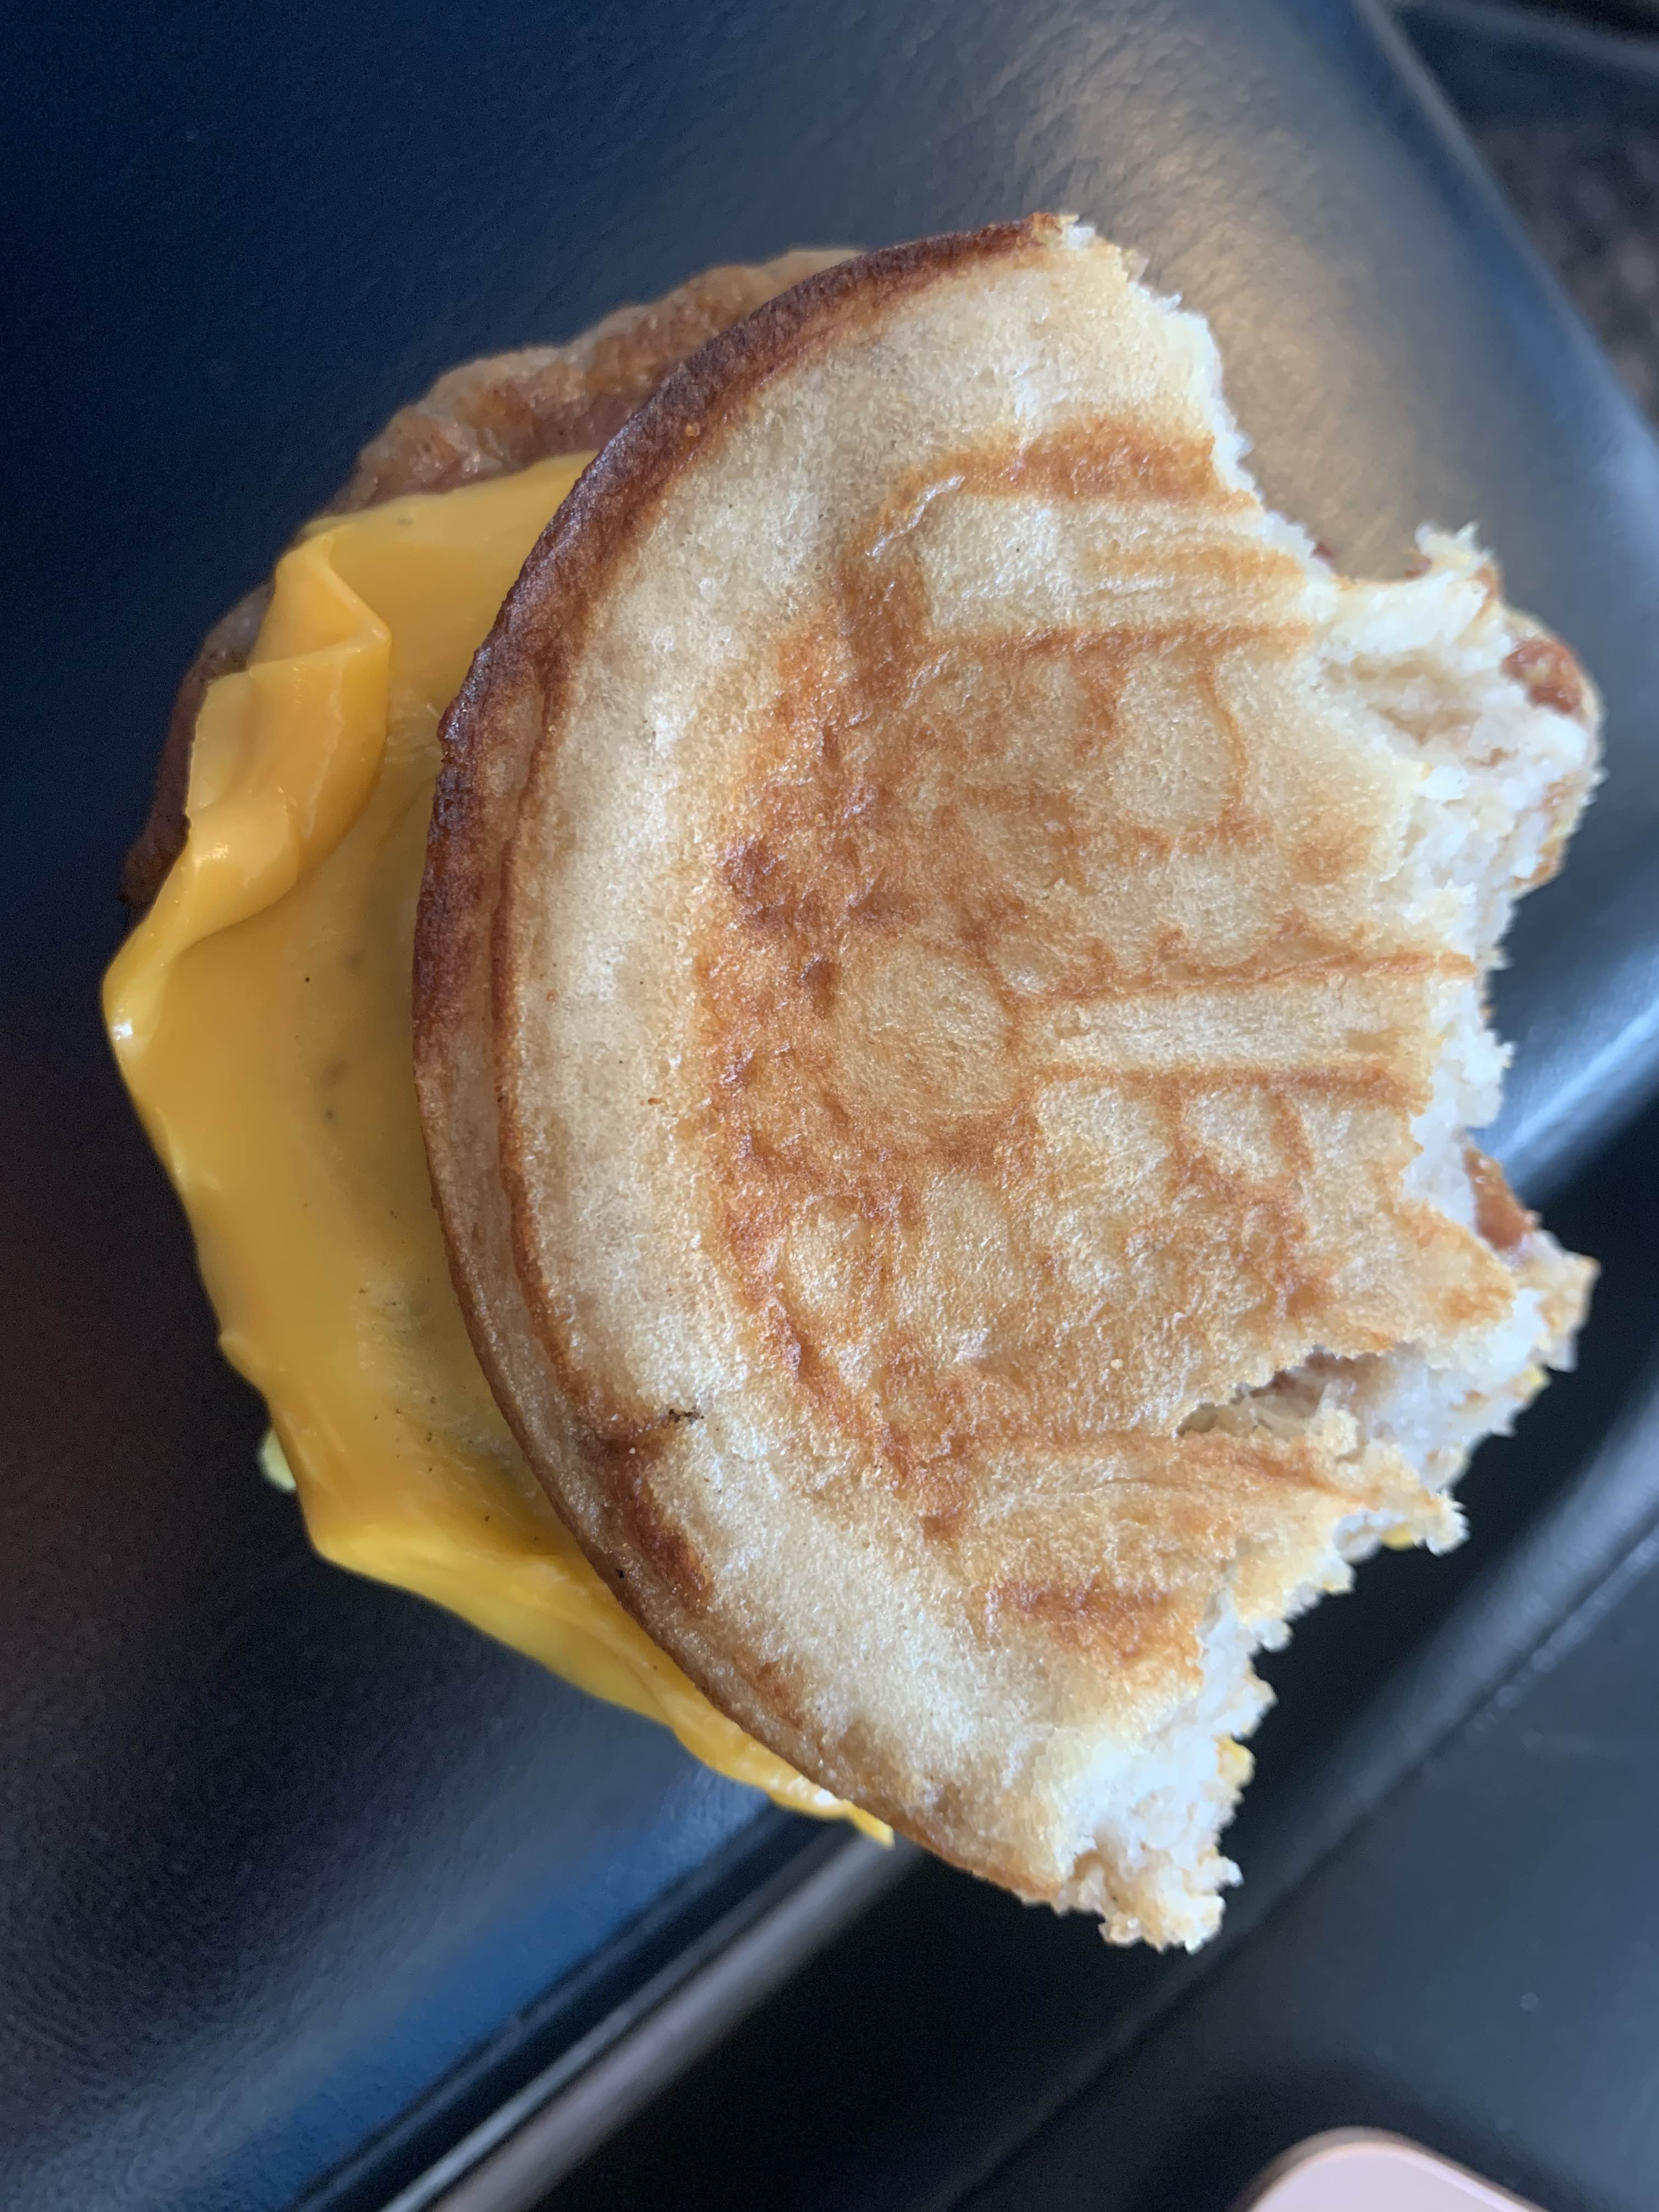
\includegraphics[width=\paperwidth]{mcdonalds-breakfast}};}
}

\begin{frame}[plain]
\end{frame}

\setbeamertemplate{background canvas}
  {
}

% insert titlepage
\begin{frame}
  \titlepage
\end{frame}

\begin{frame}
      \begin{figure}
        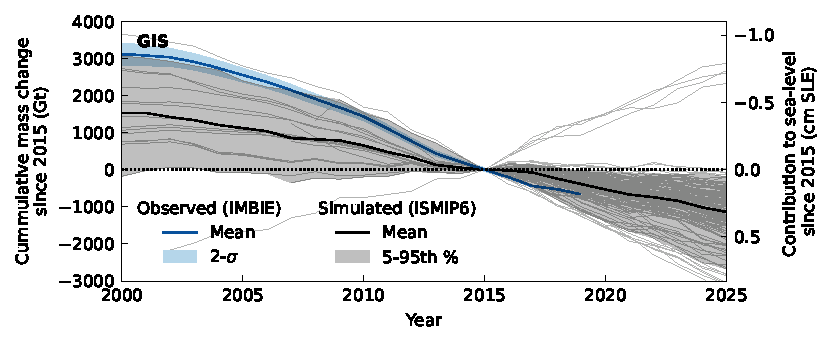
\includegraphics[width=\textwidth]{GIS_historical}
        \tiny{Aschwanden, Brinkerhoff, Bartholomaus, \& Truffer (2021)}
      \end{figure}
\end{frame}


\setbeamertemplate{background canvas}
  {
     \tikz{\node[inner sep=0pt,opacity=1.0] {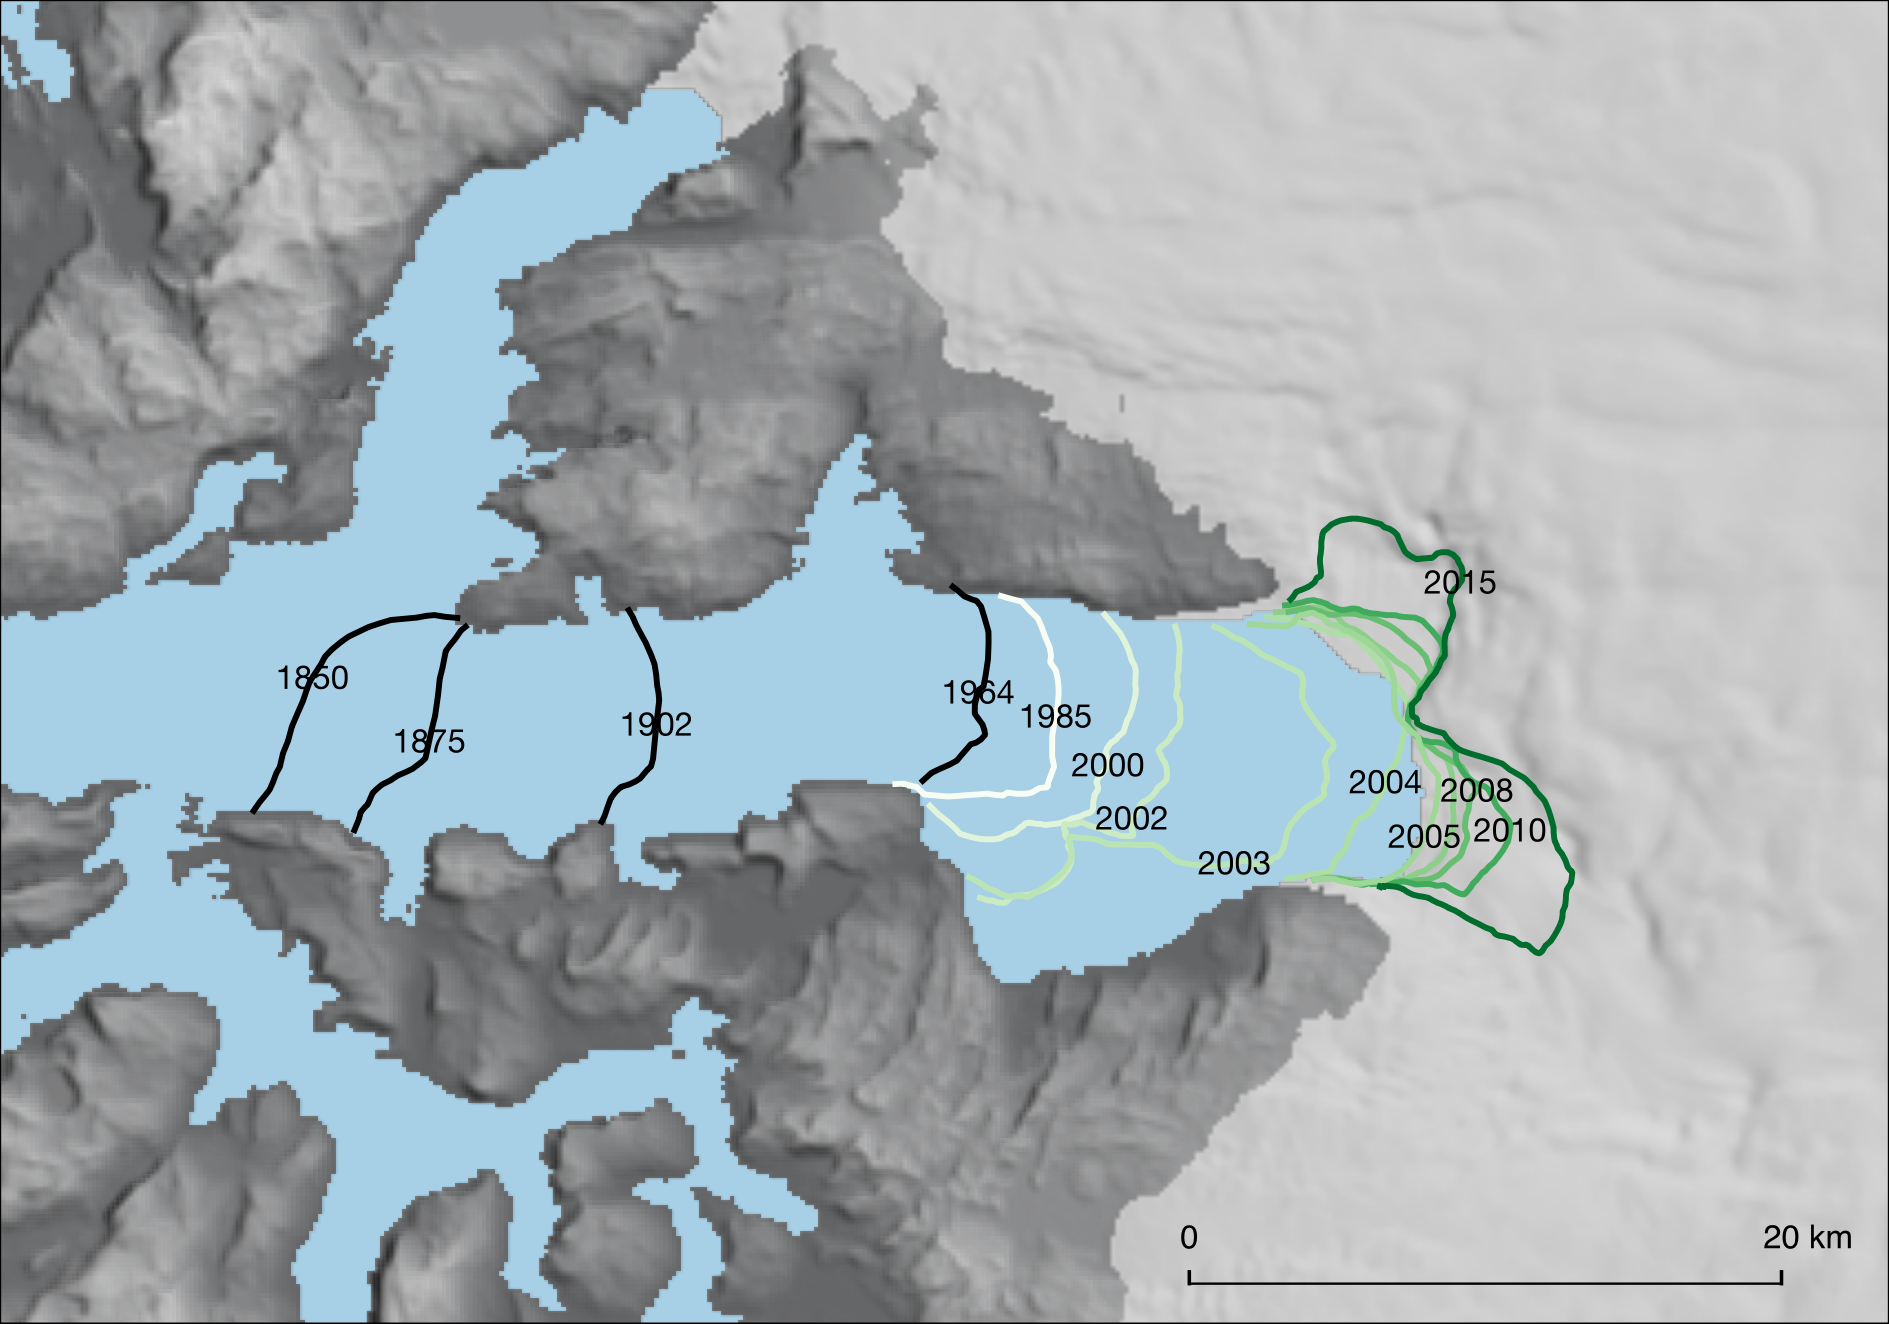
\includegraphics[width=\paperwidth]{jib-front-retreat}};}
}

\begin{frame}
\end{frame}

\setbeamertemplate{background canvas}
  {
     \tikz{\node[inner sep=0pt,opacity=1.0] {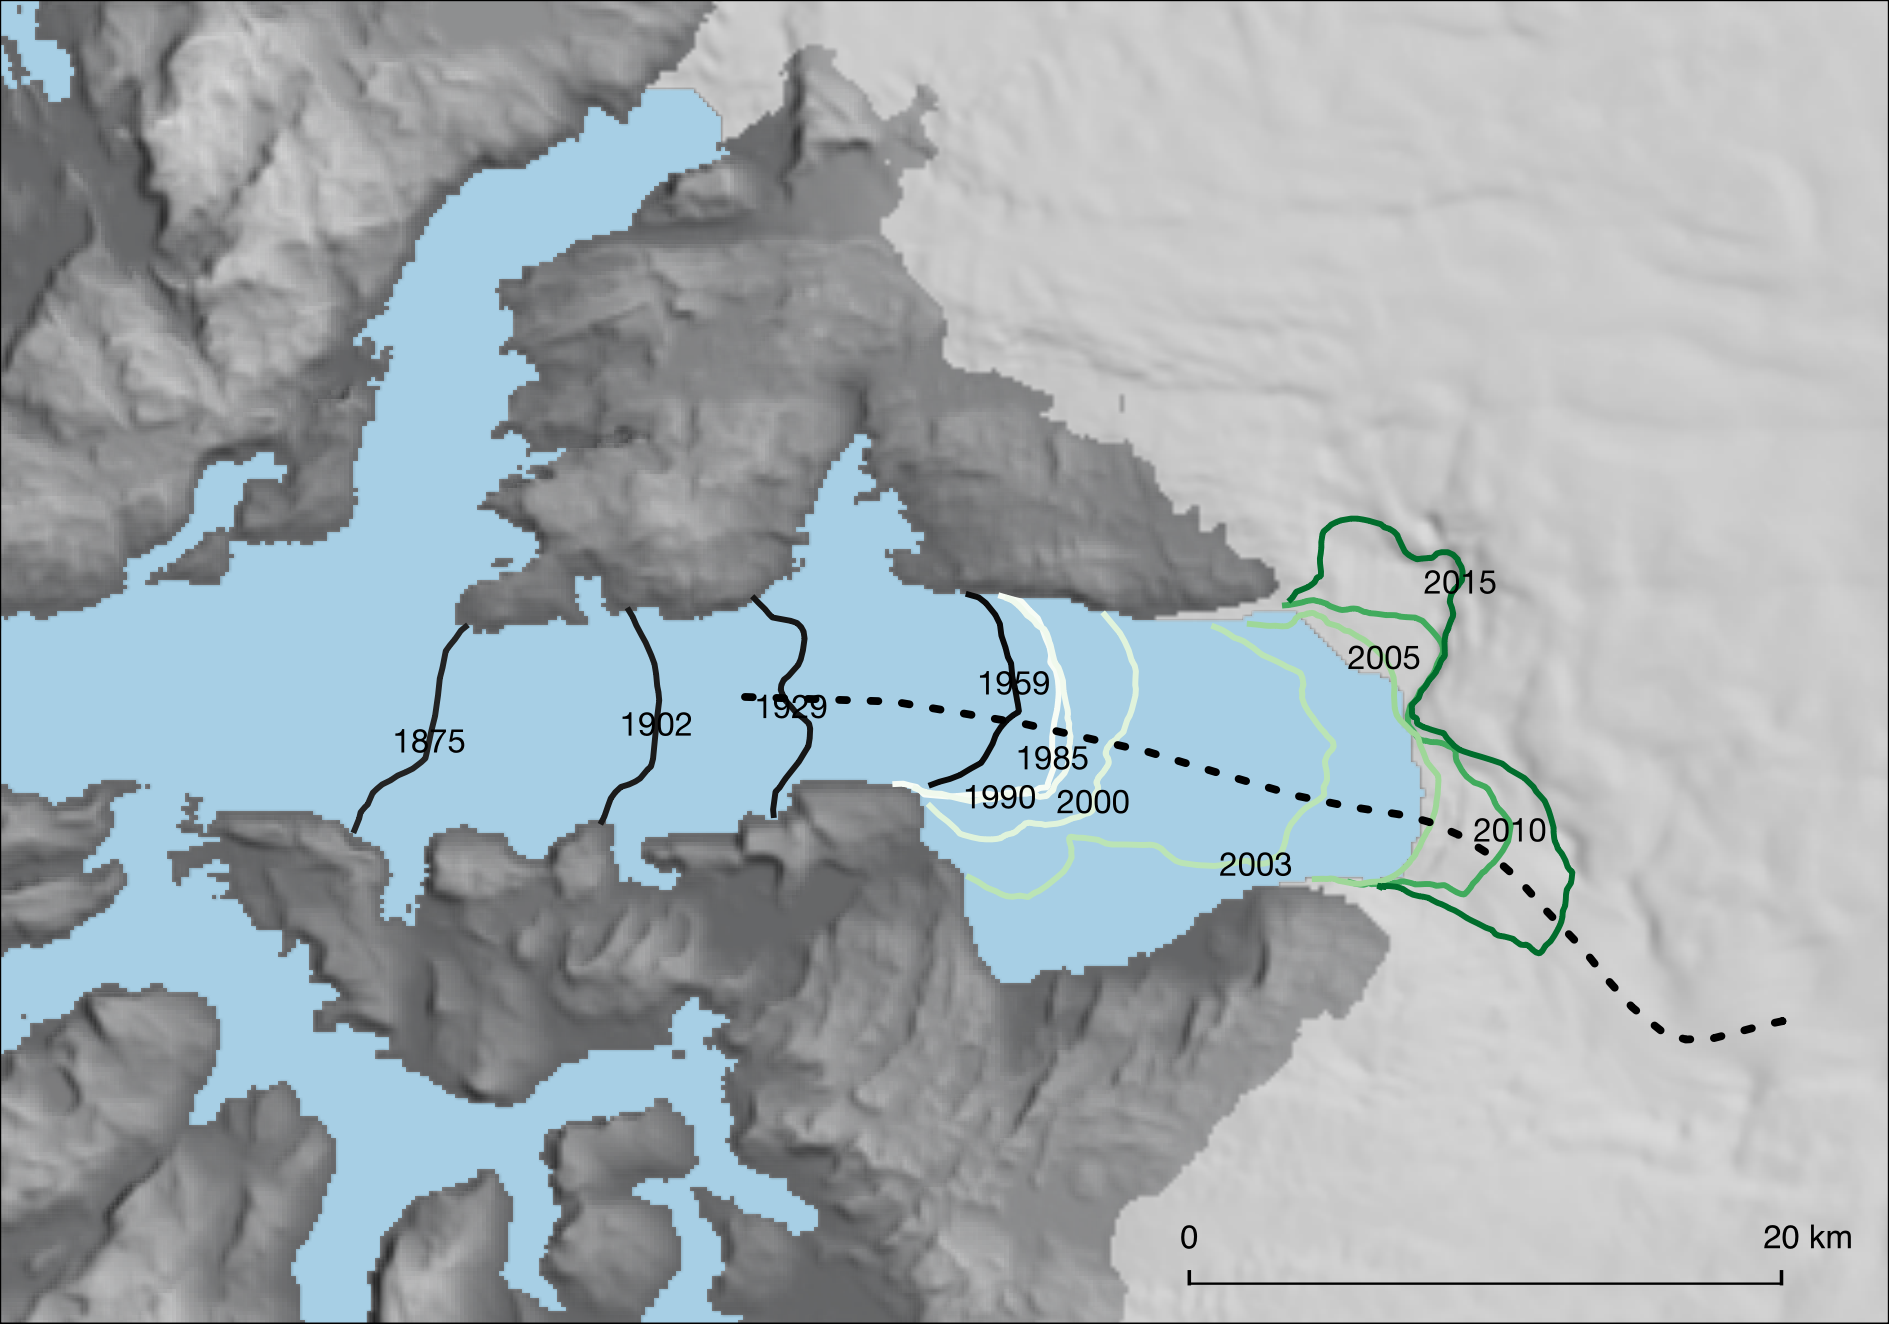
\includegraphics[width=\paperwidth]{jib-front-retreat-flowline}};}
}

\begin{frame}
\end{frame}

 \setbeamertemplate{background canvas}
  {
}

\begin{frame}[plain]
  \begin{figure}
  \includemedia[
  width=11cm,
  activate=pageopen,
  addresource=jakobshavn_flowline_id_14_hd1920.mp4,
  flashvars={loop=true&src=jakobshavn_flowline_id_14_hd1920.mp4}
  ]
  {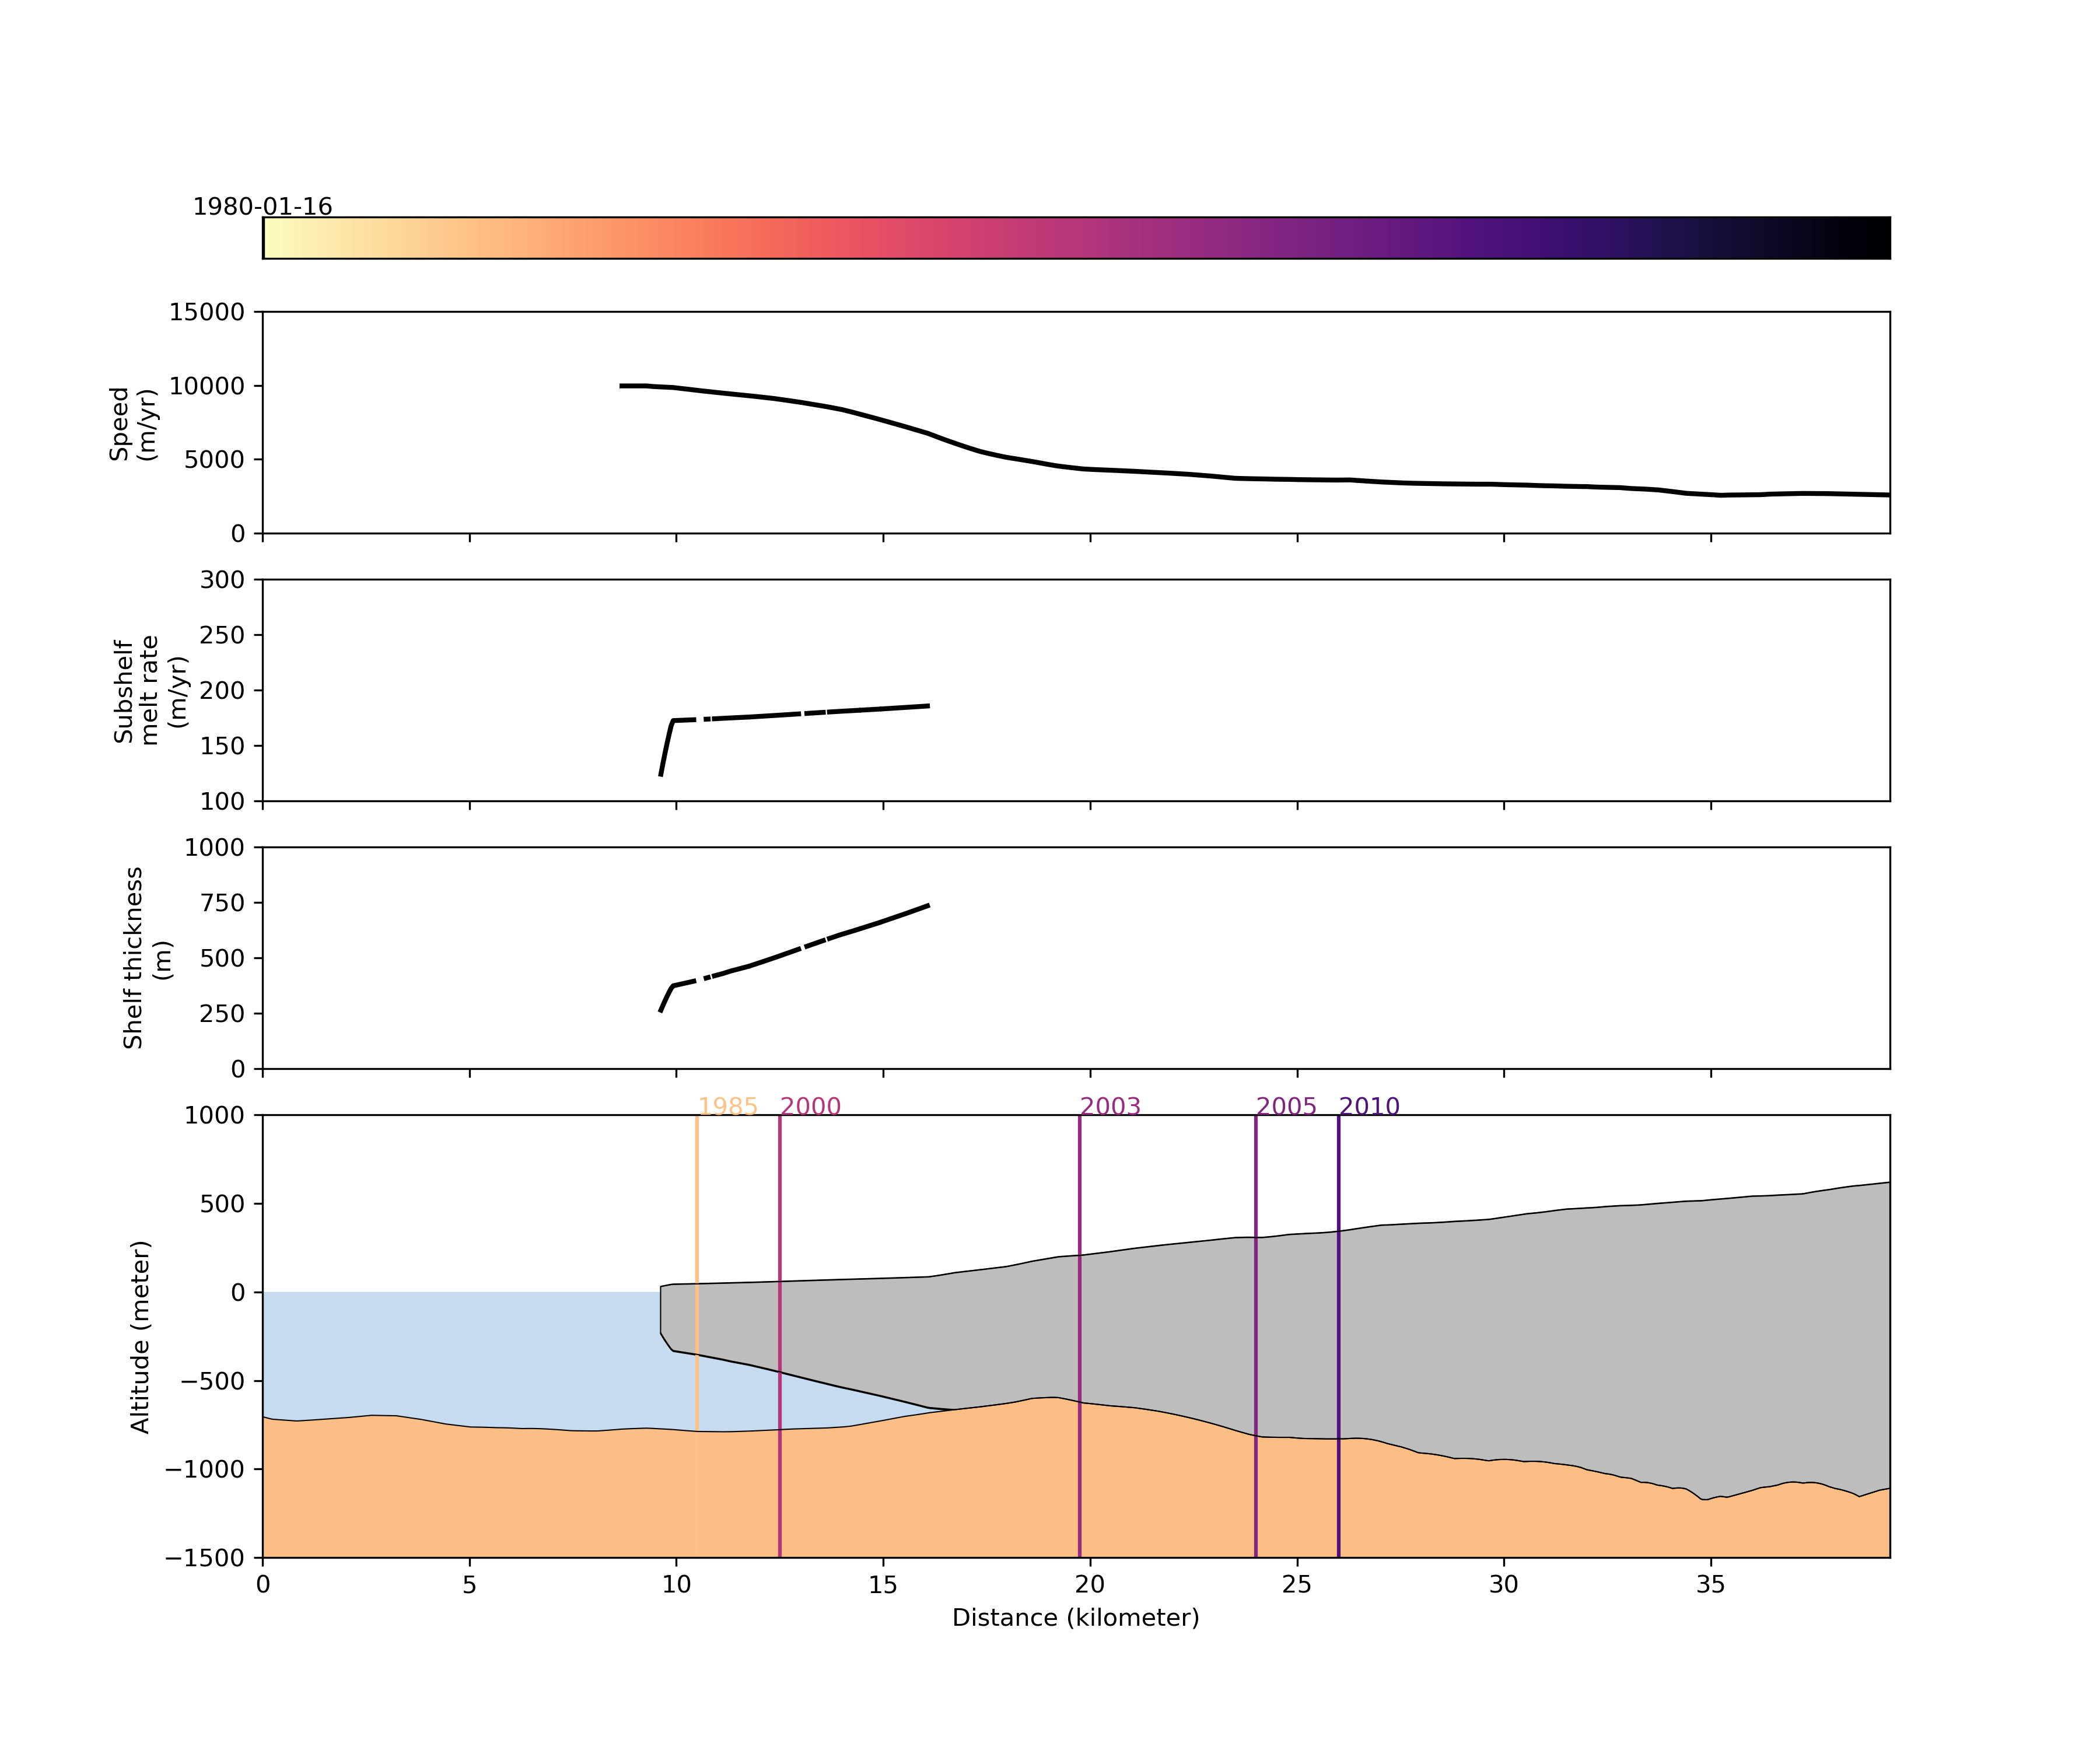
\includegraphics[width=1cm]{jakobshavn_flowline_000}}{StrobeMediaPlayback.swf}
\end{figure}
\end{frame}

\begin{frame}{}
  \begin{block}{What we get right}
  \begin{centering}
    increase in ocean forcing \alert{$\Rightarrow$} increase in subshelf melt rates \alert{$\Rightarrow$} thinning of the floating tongue \alert{$\Rightarrow$} flow acceleration
  \end{centering}
  \end{block}
  \begin{block}{What is wrong}
    \begin{itemize}
      \item floating tongue does not disintegrate
    \end{itemize}
  \end{block}
\end{frame}

  
\begin{frame}{Relevant Processes}
      \begin{figure}
        \includegraphics<1>[width=\textwidth]{jib-setup-processes}
      \end{figure}
\end{frame}



\setbeamertemplate{background canvas}
  {
     \tikz{\node[inner sep=0pt,opacity=1.0] {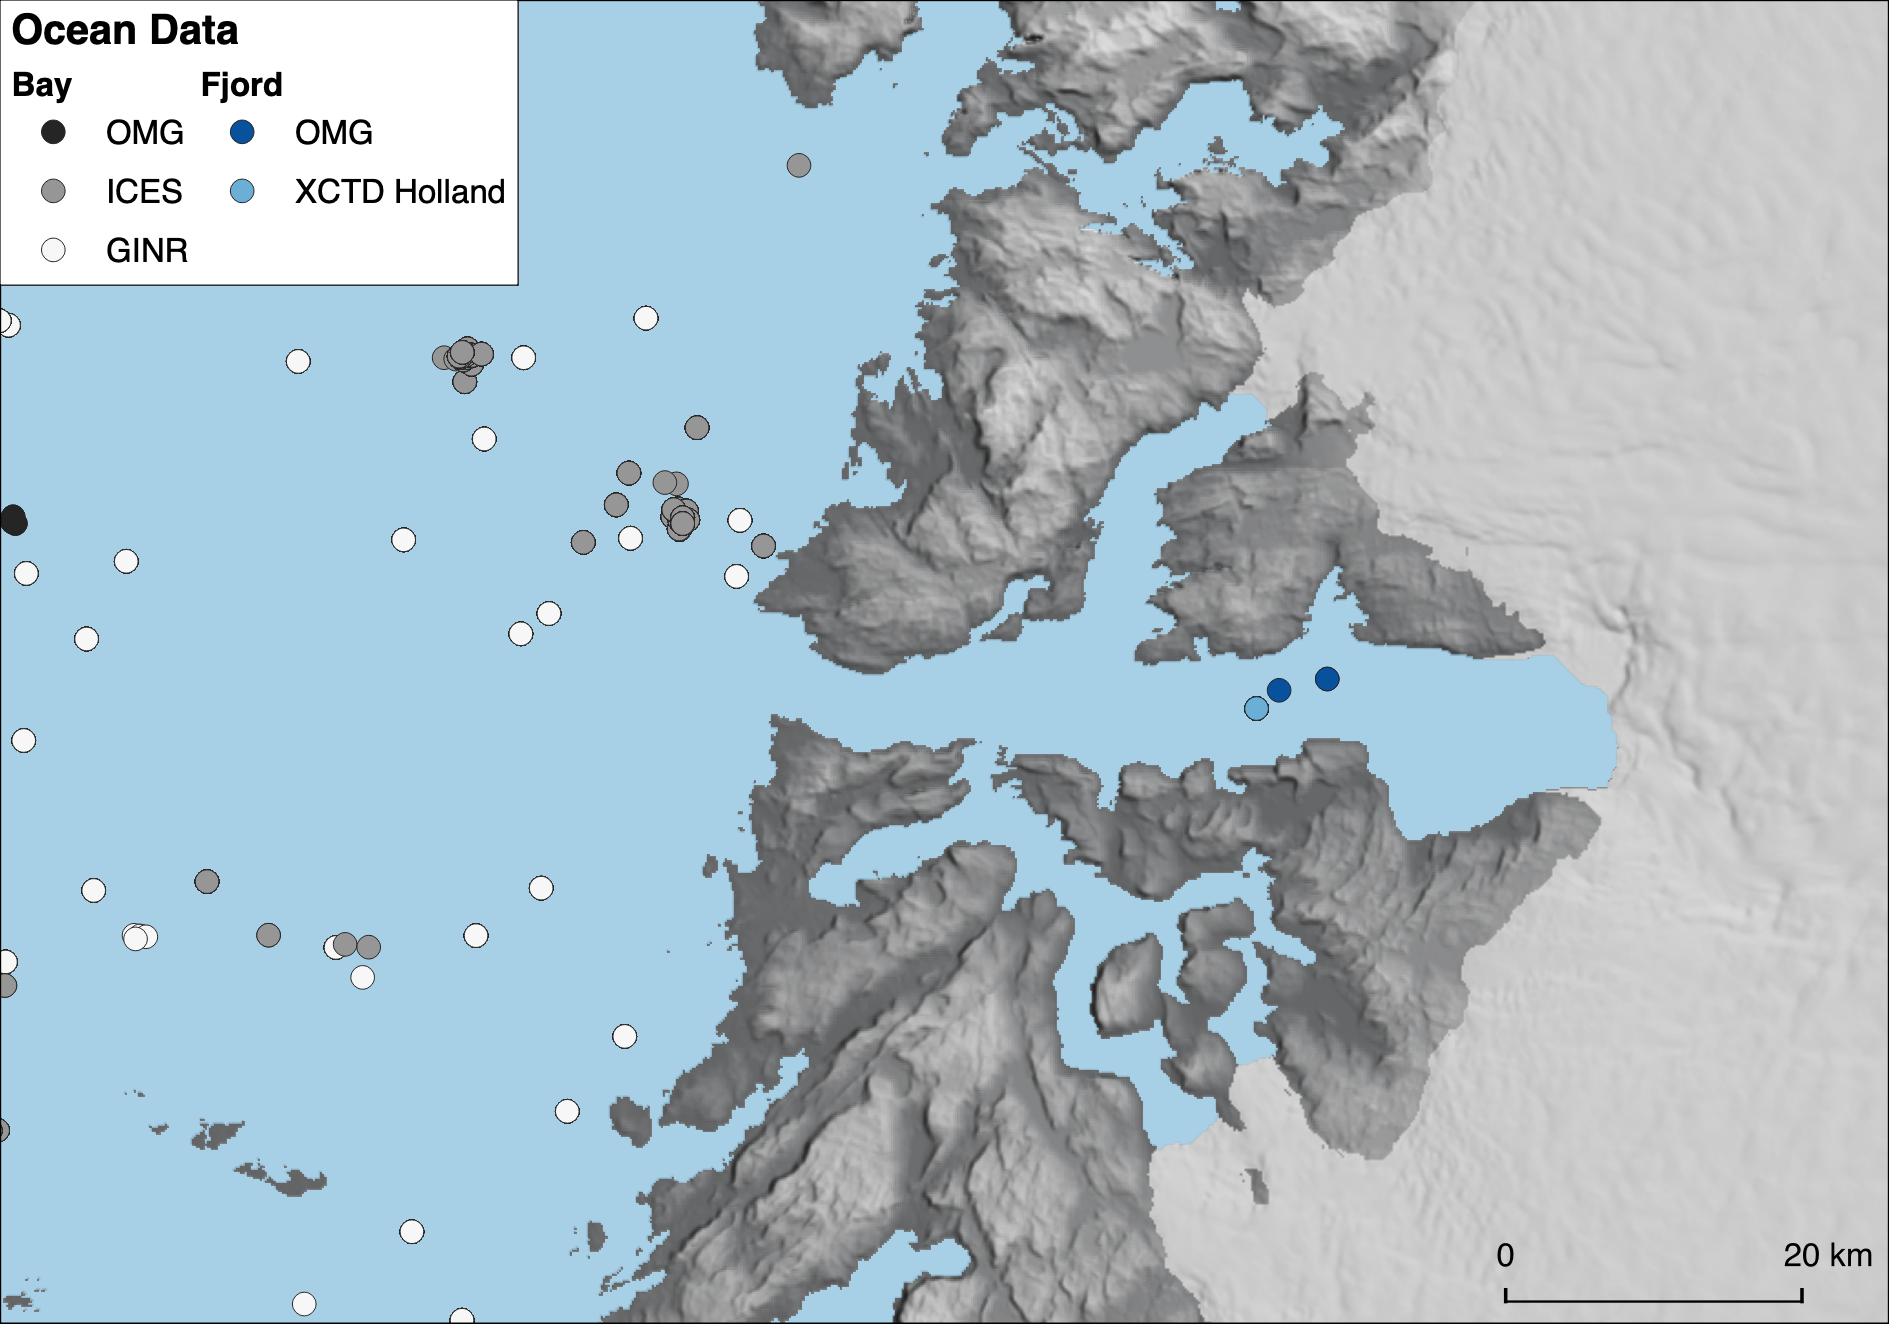
\includegraphics[width=\paperwidth]{jib-ocean-forcing-overview}};}
}
  


\begin{frame}
\end{frame}

\setbeamertemplate{background canvas}
  {
}

\begin{frame}{Ocean Forcing Reconstruction}
      \begin{figure}
        \includegraphics<1>[height=0.8\textheight]{jib_ocean_observation_categorical_1980_2020}
        \includegraphics<2>[height=0.8\textheight]{jib_ocean_forcing_1980_2020_normalized}
      \end{figure}
\end{frame}

  
  \begin{frame}{Ensemble simulations}
    72 ensemble members drawn from parameter distributions relating to
  \begin{itemize}
  \item damage mechanics (5)
  \item calving (2)
  \end{itemize}
      \begin{figure}
        \includegraphics<1>[width=\textwidth]{jib-setup}
      \end{figure}
\end{frame}

  
  
\begin{frame}{1985}
  \begin{columns}[t]
    \begin{column}{2cm}
      \begin{figure}
        \includegraphics<1>[width=\textwidth]{roman-motyka-yakutat}
        \includegraphics<2>[width=\textwidth]{pism_logo_v2_transp}
      \end{figure}
    \end{column}
    \begin{column}{11cm}
      \begin{figure}
        \includegraphics<1>[width=\textwidth]{jib_1985_speed_observed}
        \includegraphics<2>[width=\textwidth]{jib_1985_speed_simulated}
      \end{figure}
    \end{column}
  \end{columns}
\end{frame}



\begin{frame}{Termini 1985}
      \begin{figure}
        \includegraphics<1>[width=.975\textwidth]{jib-fronts-1985}
      \end{figure}
\end{frame}

\begin{frame}{Termini 2020}
      \begin{figure}
        \includegraphics<1>[width=.975\textwidth]{jib-fronts-2020}
      \end{figure}
\end{frame}


\begin{frame}{Grounding line flux}
      \begin{figure}
        \includegraphics<1>[width=\textwidth]{jib_total_grounding_line_flux}
      \end{figure}
\end{frame}


\begin{frame}{What we get right}
  \begin{centering}
    increase in ocean forcing \alert{$\Rightarrow$} increase in subshelf melt rates \alert{$\Rightarrow$} thinning of the floating tongue \alert{$\Rightarrow$} flow acceleration
  \end{centering}
\end{frame}

\begin{frame}{What is missing}
      \begin{minipage}[t][.9\textheight][t]{.9\textwidth}
  \begin{block}{Calving}
    \begin{itemize}
    \item Downs, Brinkerhoff, Morlighem (2022): 
a simple stochastic model relating surface runoff rates and calving threshold is able to reproduce observations with respect to both mean position and characteristic temporal variability.    \end{itemize}
      \begin{figure}
        \includegraphics<2->[width=.9\textwidth]{jib-runoff-1980-2020.pdf}
      \end{figure}
  \end{block}

      \end{minipage}
\end{frame}


 \setbeamertemplate{background canvas}
  {
}

\begin{frame}[plain]
  \begin{figure}
  \includemedia[
  width=11cm,
  activate=pageopen,
  addresource=jakobshavn_flowline_id_14_hd1920.mp4,
  flashvars={src=jakobshavn_flowline_id_14_hd1920.mp4}
  ]
  {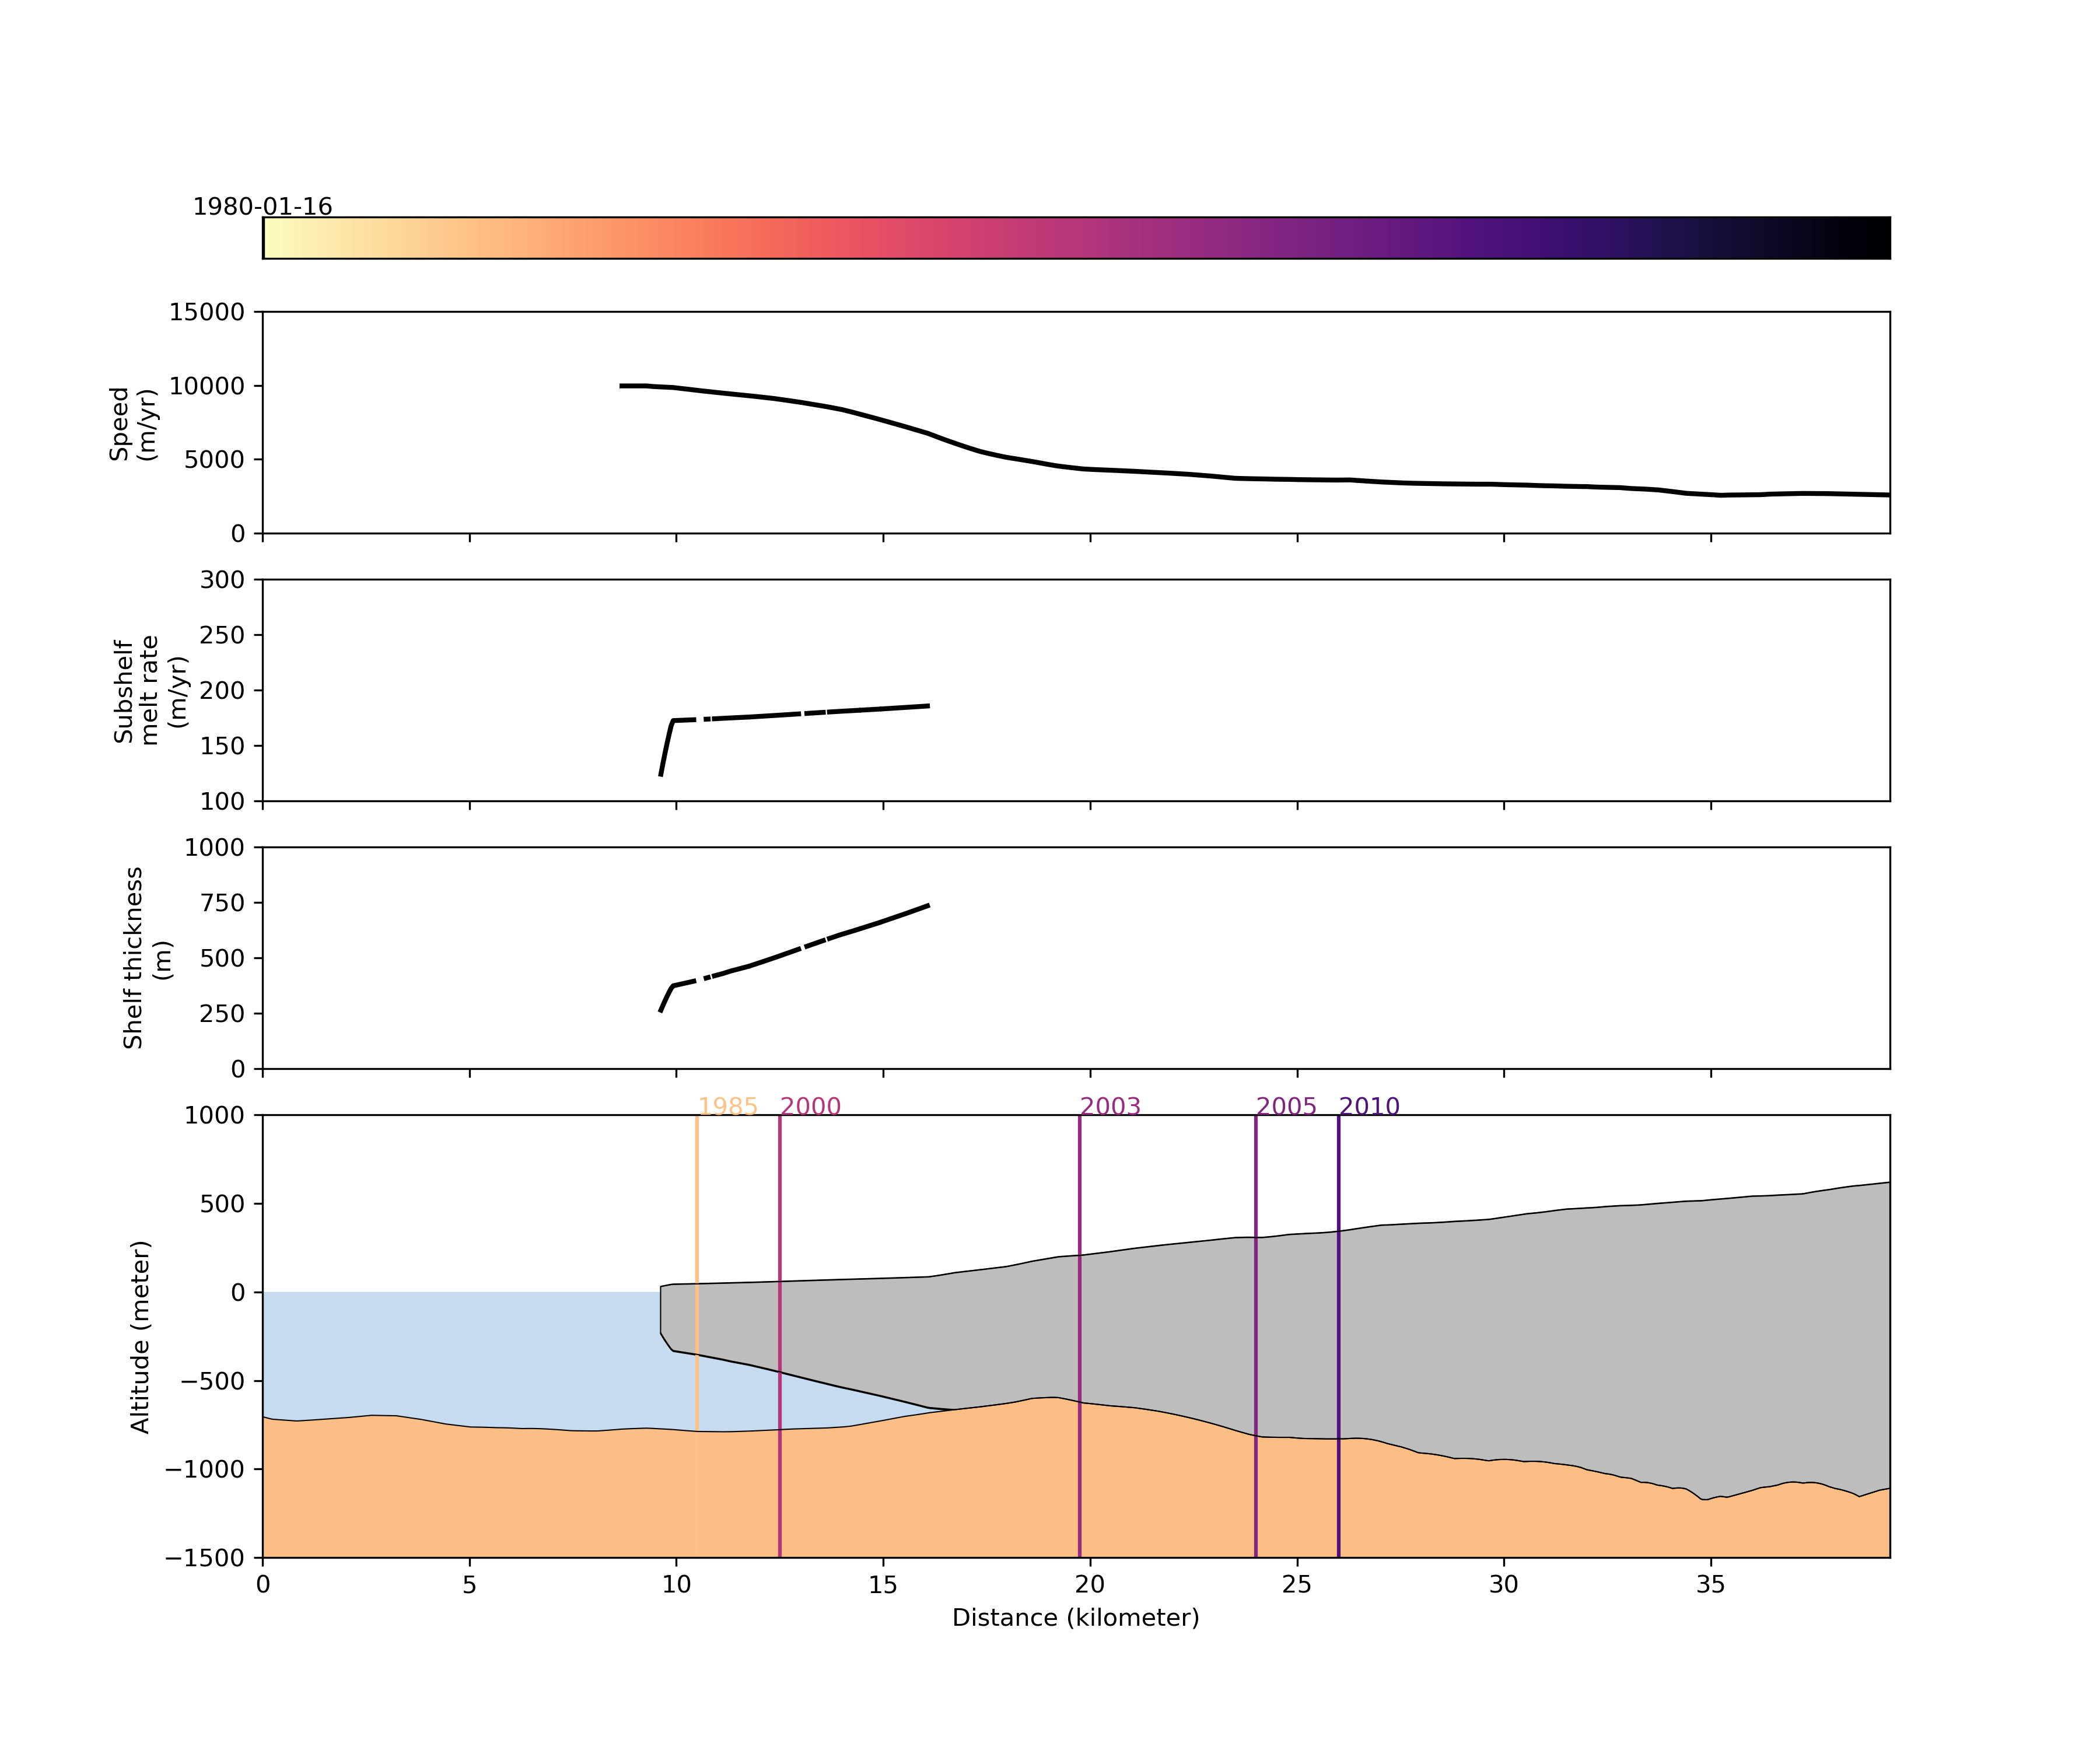
\includegraphics[width=11cm]{jakobshavn_flowline_000}}{StrobeMediaPlayback.swf}
\end{figure}
\end{frame}


\end{document}
